% Pour faire une référence d'une annexe
% (Annexe \ref{sec:nomsection} page~\pageref{sec:nomsection})

\section{Exemple de texte neumé}
\label{sec:exempleTexteNeume}
\begin{figure}[H]
	\centering
	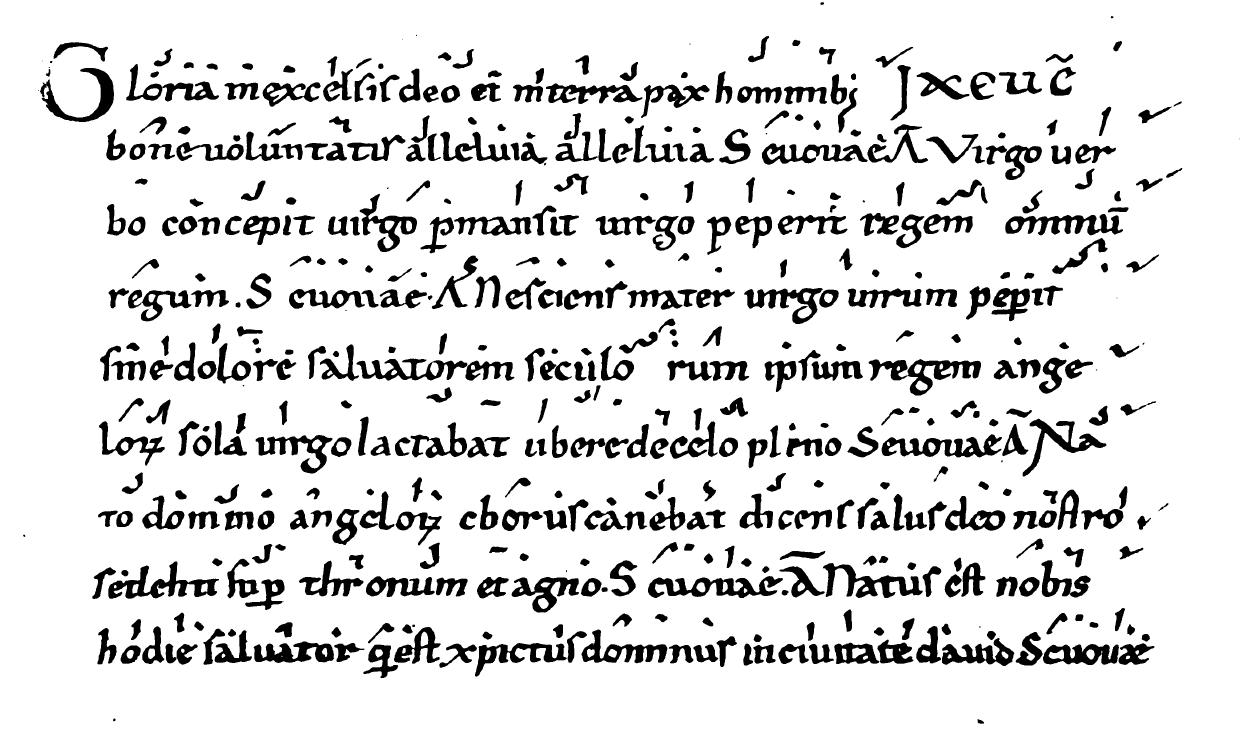
\includegraphics[keepaspectratio=true, width=\textwidth]{Annexes/i/neumes.jpg}
	\caption{Exemple de texte neumé  }
	\medskip
	\small	
	Source : 1774, Martin Gerbert, \textit{De cantu et musica sacra a prima Ecclesiae aetate usque ad praesens Tempus}, St. Blasien, Typis San-Blasianis, t. I, t. II. - \textit{Les neumes sont les symboles inscrient au-dessus des mots du chant liturgique (ici le chant} Gloria \textit{de l'ordinaire de la messe).}
	\label{fig:neumes}
\end{figure}
\clearpage

\section{La notation carrée}
\label{sec:exempleNotationCarree}
\begin{figure}[H]
	\centering
	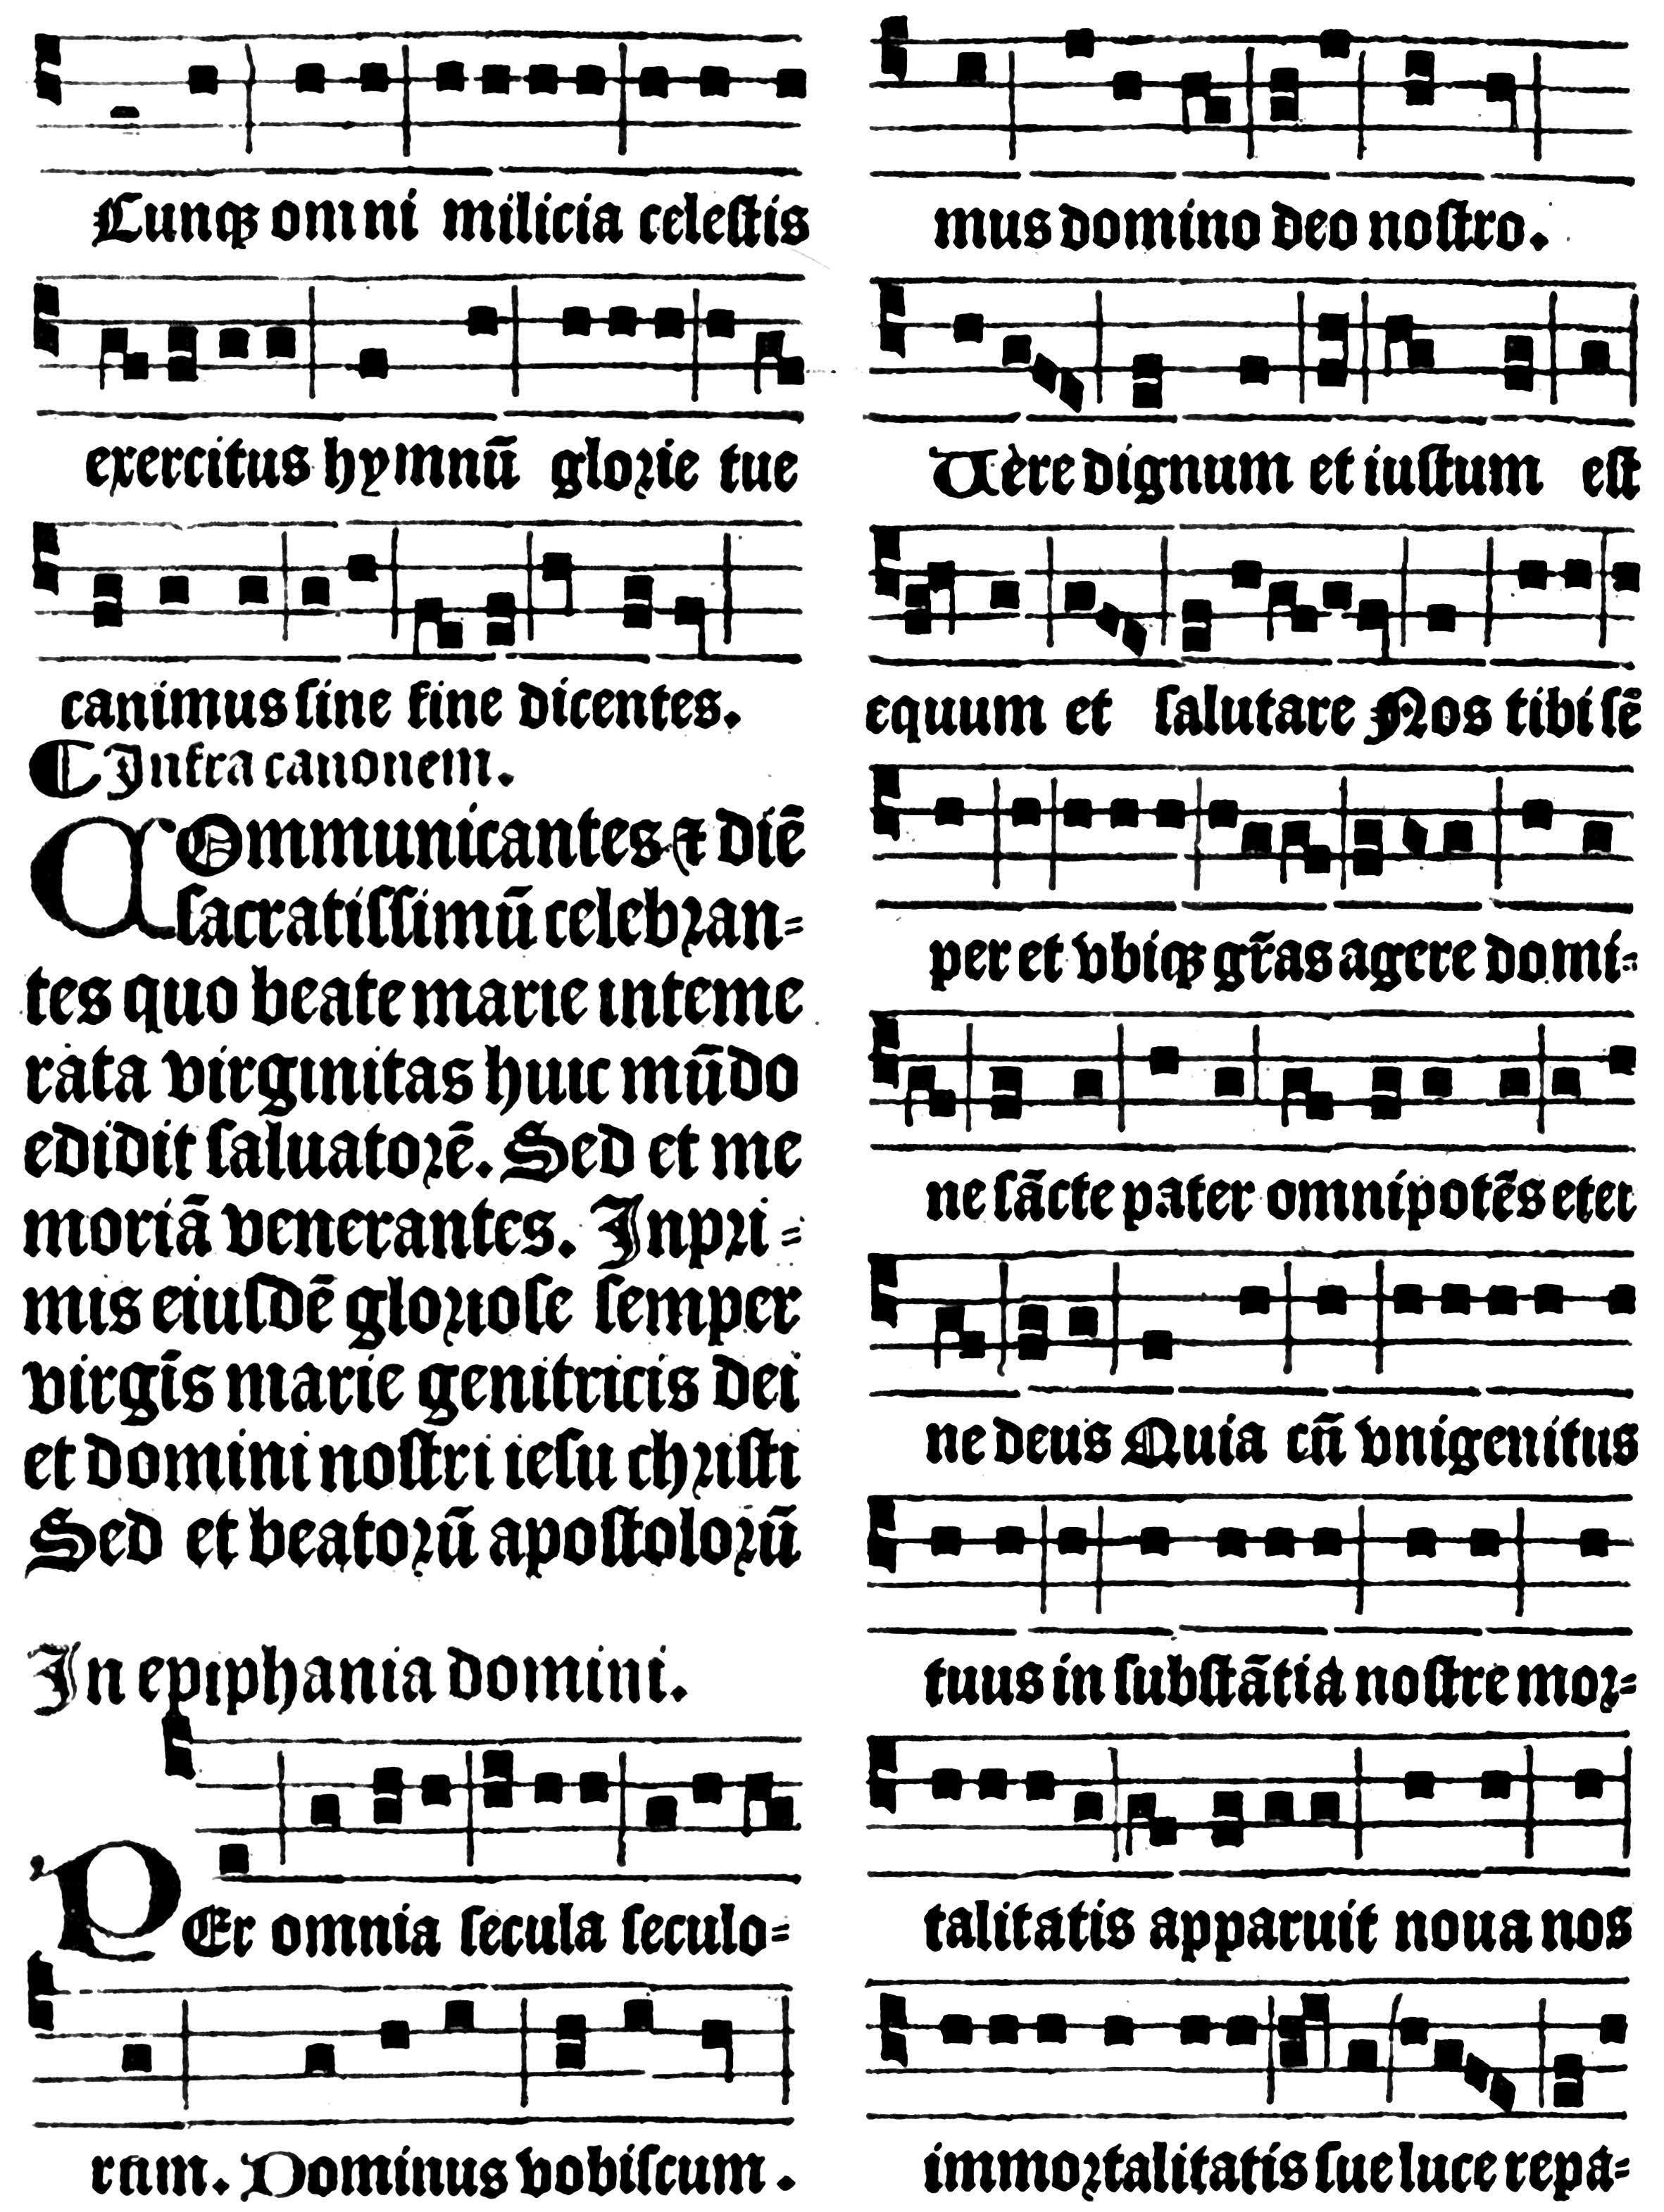
\includegraphics[keepaspectratio=true, width=\textwidth]{Annexes/i/notationCarree.jpg}
	\caption{Exemple de notation carrée "imprimée"}
	\medskip
	\small
	Source : 1499, Jean Highman, \textit{Missale Leodiense}, Paris - \textit{Les notes sont représentées en notation carrée toujours au-dessus du texte chanté.}
	\label{fig:notationCarree}
\end{figure}
\clearpage

\section{La notation épurée de l'époque baroque}
\label{sec:exempleMusiqueBaroque}
\begin{figure}[H]
	\centering
	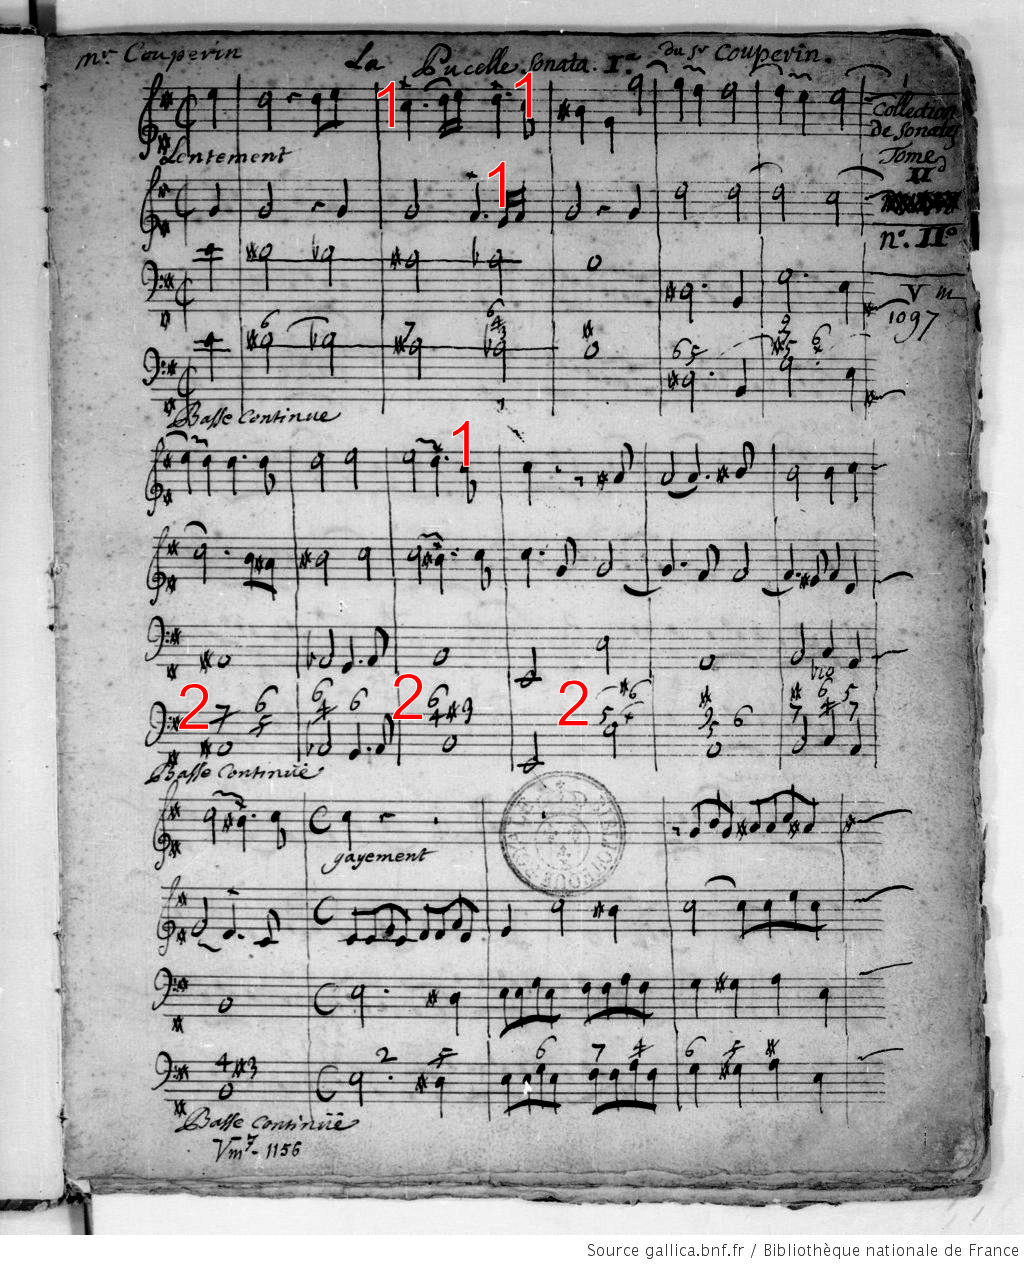
\includegraphics[keepaspectratio=true, width=\textwidth]{Annexes/i/exempleMusiqueBaroque.jpeg}
	\caption{Extrait de la pièce \textit{La Pucelle}, par François Couperin, 1690-1710}
	\medskip
	\small
	\textit{Source : Bibliothèque nationale de France, département Musique, VM7-1156} 	
	\label{fig:exempleMusiqueBaroque}
\end{figure}
\clearpage

\section{La notation de l'interprétation}
\label{sec:exempleNotationInterpretation}
\begin{figure}[H]
	\centering
	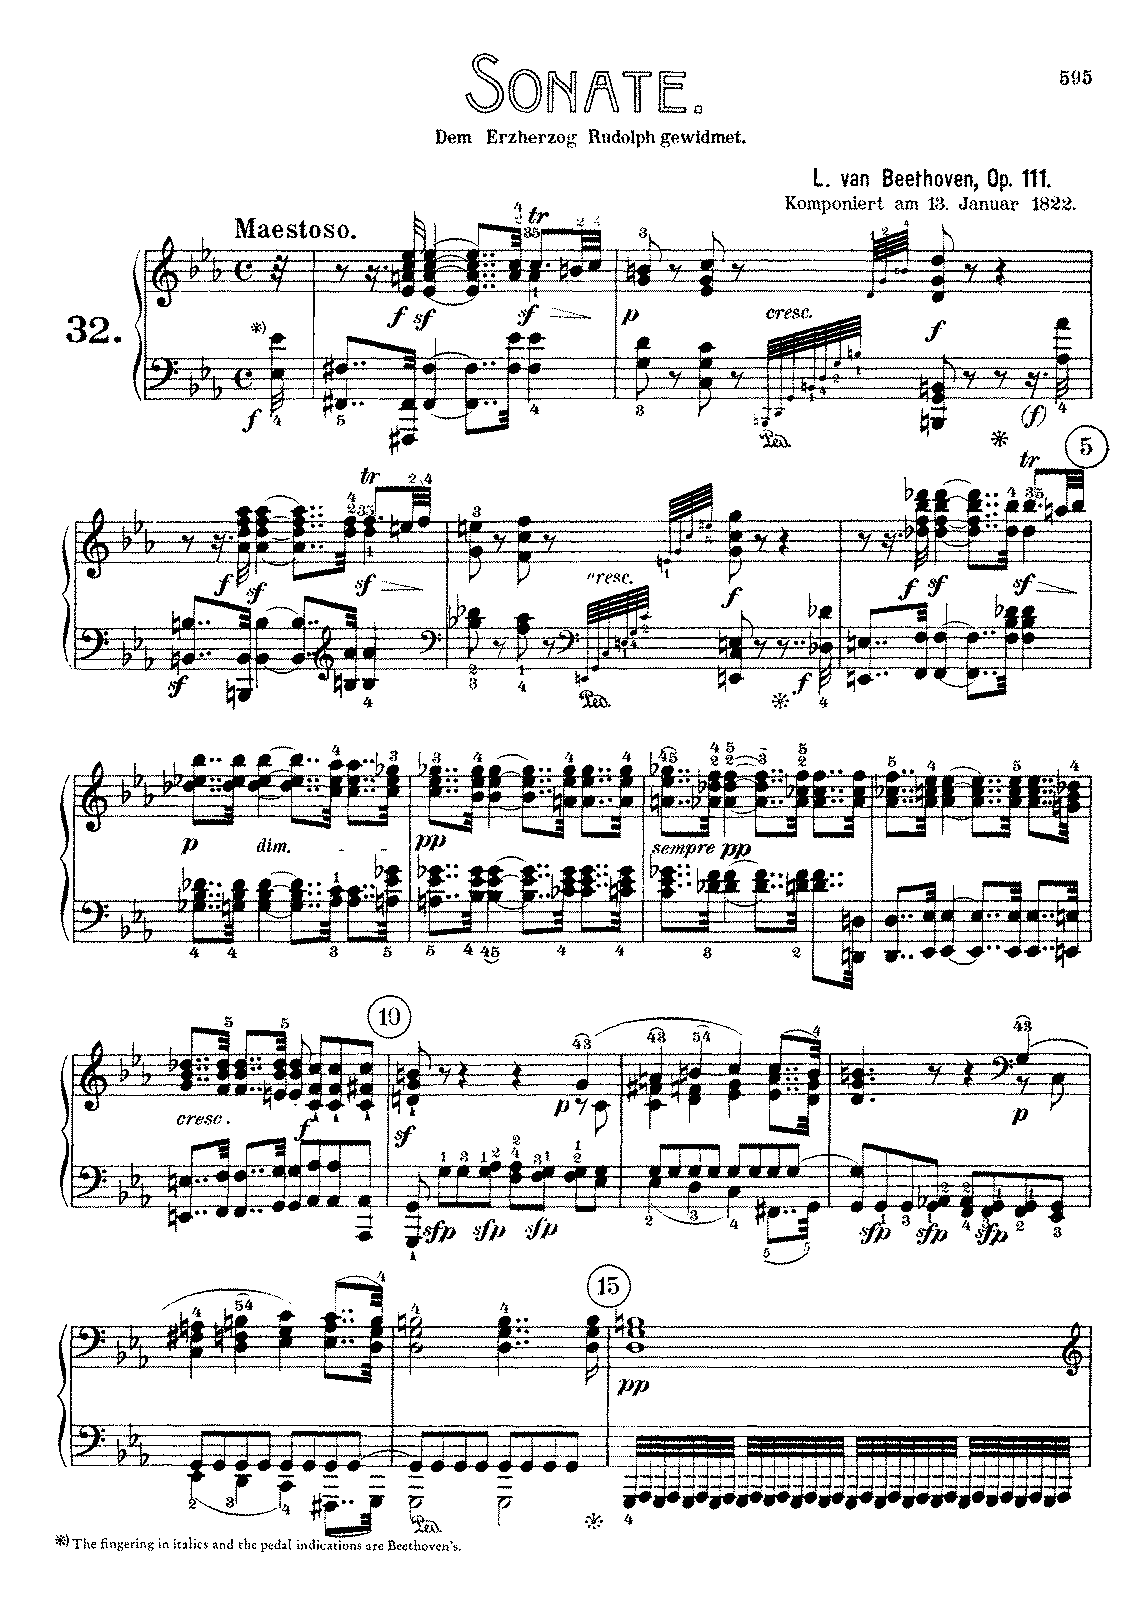
\includegraphics[keepaspectratio=true, width=0.9\textwidth]{Annexes/i/exempleNotationInterpretation.png}
	\caption{Extrait de la \textit{Sonate pour piano, N.32, Opus 111}, Ludwig van Beethoven, 1821-1822}
	\medskip
	\small
	\textit{Source : IMSLP, Petrucci Music Library} 	
	\label{fig:exempleNotationInterpretation}
\end{figure}

\section{Exemple de partition graphique du XXème siècle}
\label{sec:exempleAnestisLogothetis}
\begin{figure}[H]
	\centering
	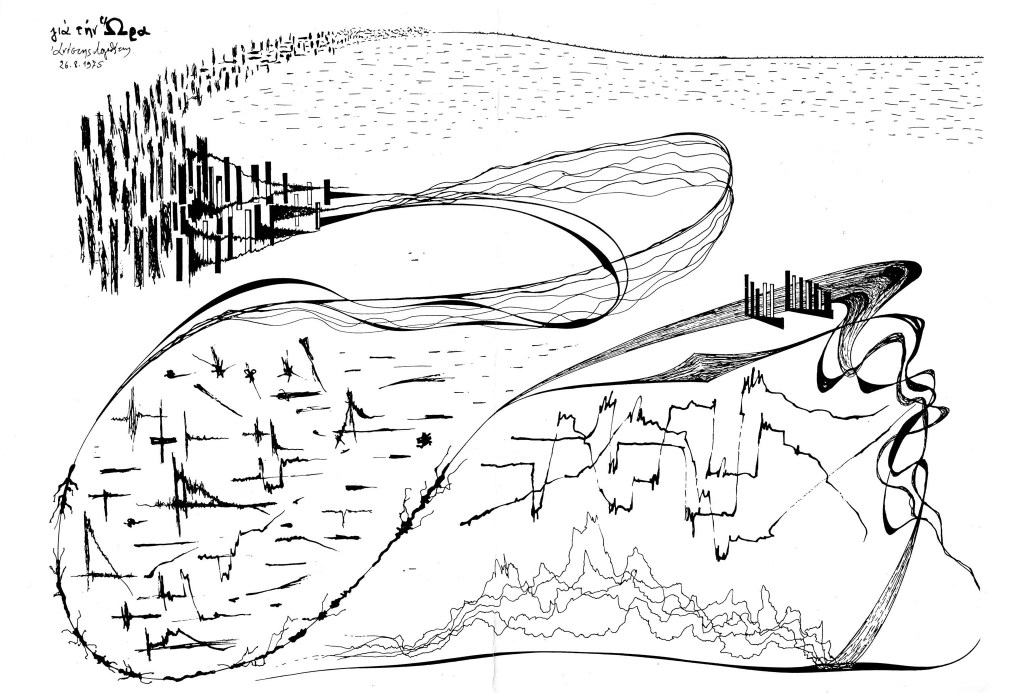
\includegraphics[keepaspectratio=true, width=0.9\textwidth]{Annexes/i/exempleAnestisLogothetis.jpg}
	\caption{Partition de \textit{Ghia tin ora} (Pour l'heure), Anestis Logothetis, 1975}
	\medskip
	\small
	\textit{Source : \url{http://schlachten.org/artist/logothetis-ensemble/}} 	
	\label{fig:exempleAnestisLogothetis}
\end{figure}
\clearpage

\section{Notation du geste dans la musique contemporaine}
\label{sec:exempleKarimHaddad}
\begin{figure}[H]
	\centering
	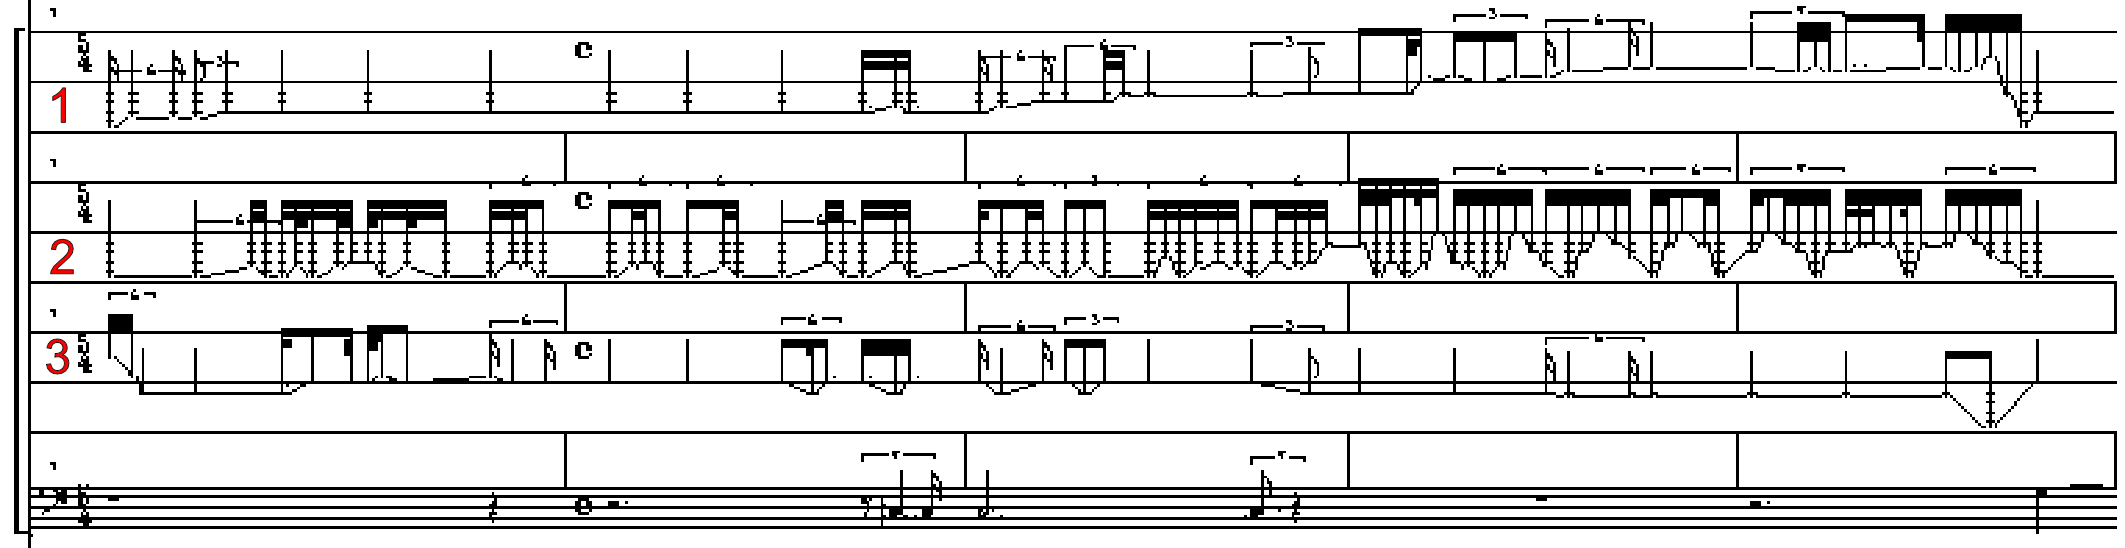
\includegraphics[keepaspectratio=true, width=\textwidth]{Annexes/i/exempleKarimHaddad.png}
	\caption{Fragment de la pièce \textit{In lieblicher Blaue…}, Karim Haddad}
	\medskip
	\small
	\label{fig:exempleKarimHaddad}
\end{figure}
\clearpage

\section{Notation de la spatialisation du son dans la musique contemporaine}
\label{sec:exempleAlirezaFarhang}
\begin{figure}[H]
	\centering
	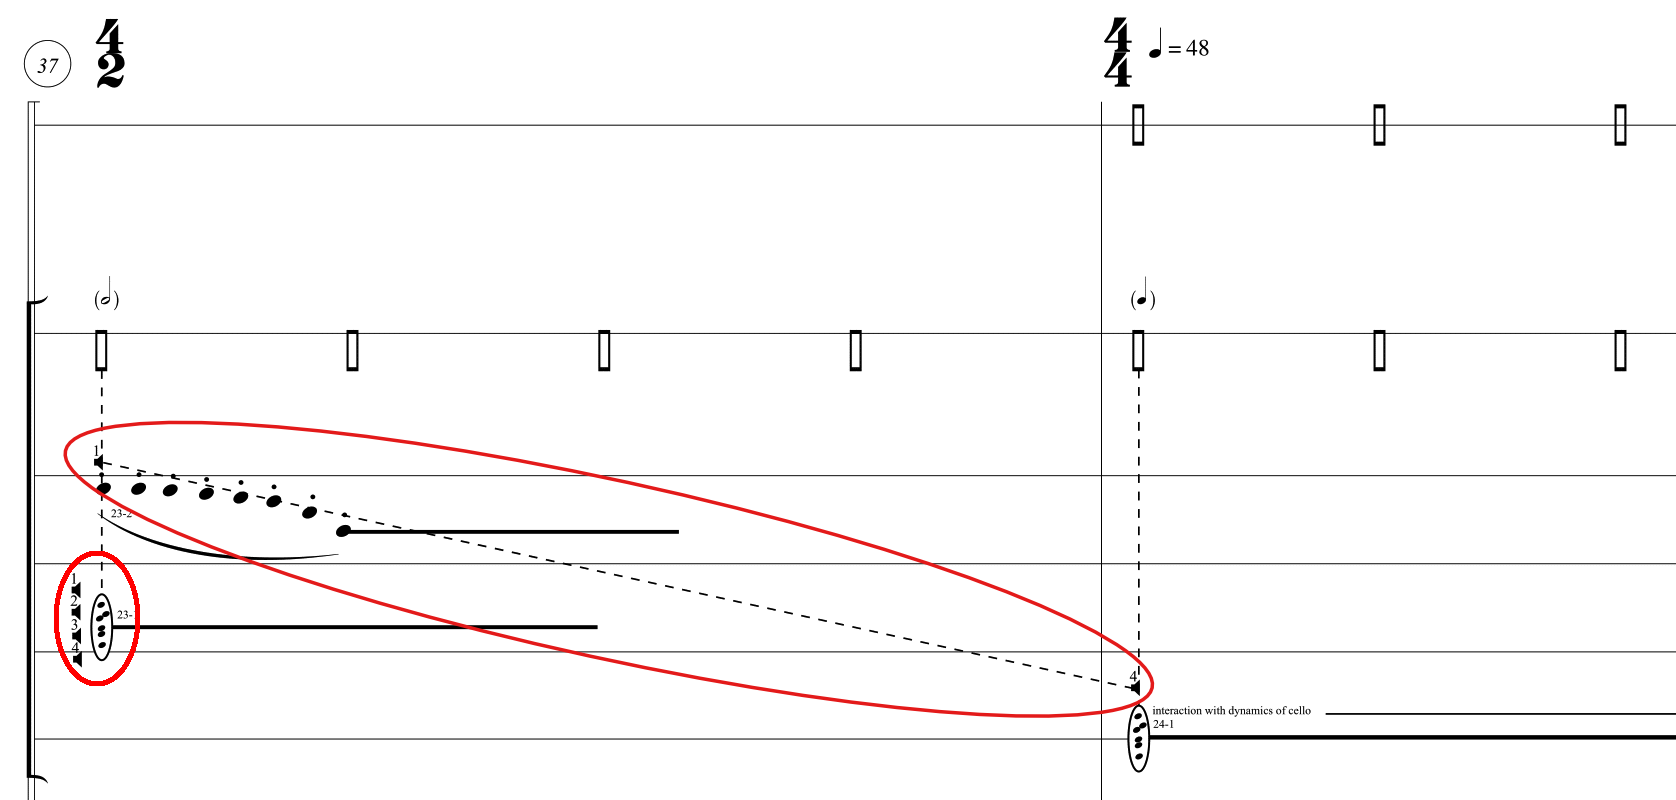
\includegraphics[keepaspectratio=true, width=\textwidth]{Annexes/i/exempleAlirezaFarhang.png}
	\caption{Fragment de la pièce \textit{Tak Sîm}, Alireza Farhang, 2012}
	\medskip
	\small
	\label{fig:exempleAlirezaFarhang}
\end{figure}
\clearpage

\section{Notation des effets appliqués au son dans la musique contemporaine}
\label{sec:exempleStockhausen}
\begin{figure}[H]
	\centering
	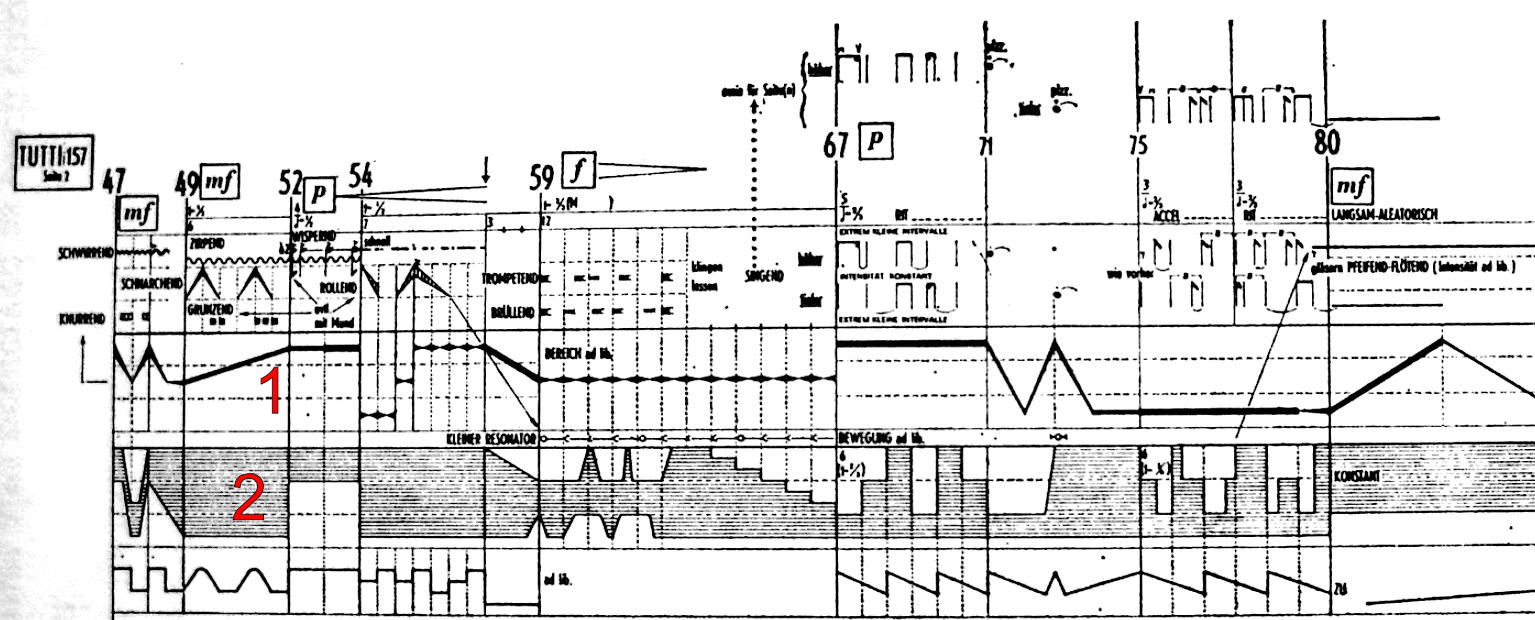
\includegraphics[keepaspectratio=true, width=0.8\textwidth]{Annexes/i/exempleStockhausen.jpg}
	\caption{Fragment de la pièce \textit{Tutti 157}, Karlheinz Stockhausen, 1964}
	\medskip
	\small
	\label{fig:exempleStockhausen}
\end{figure}


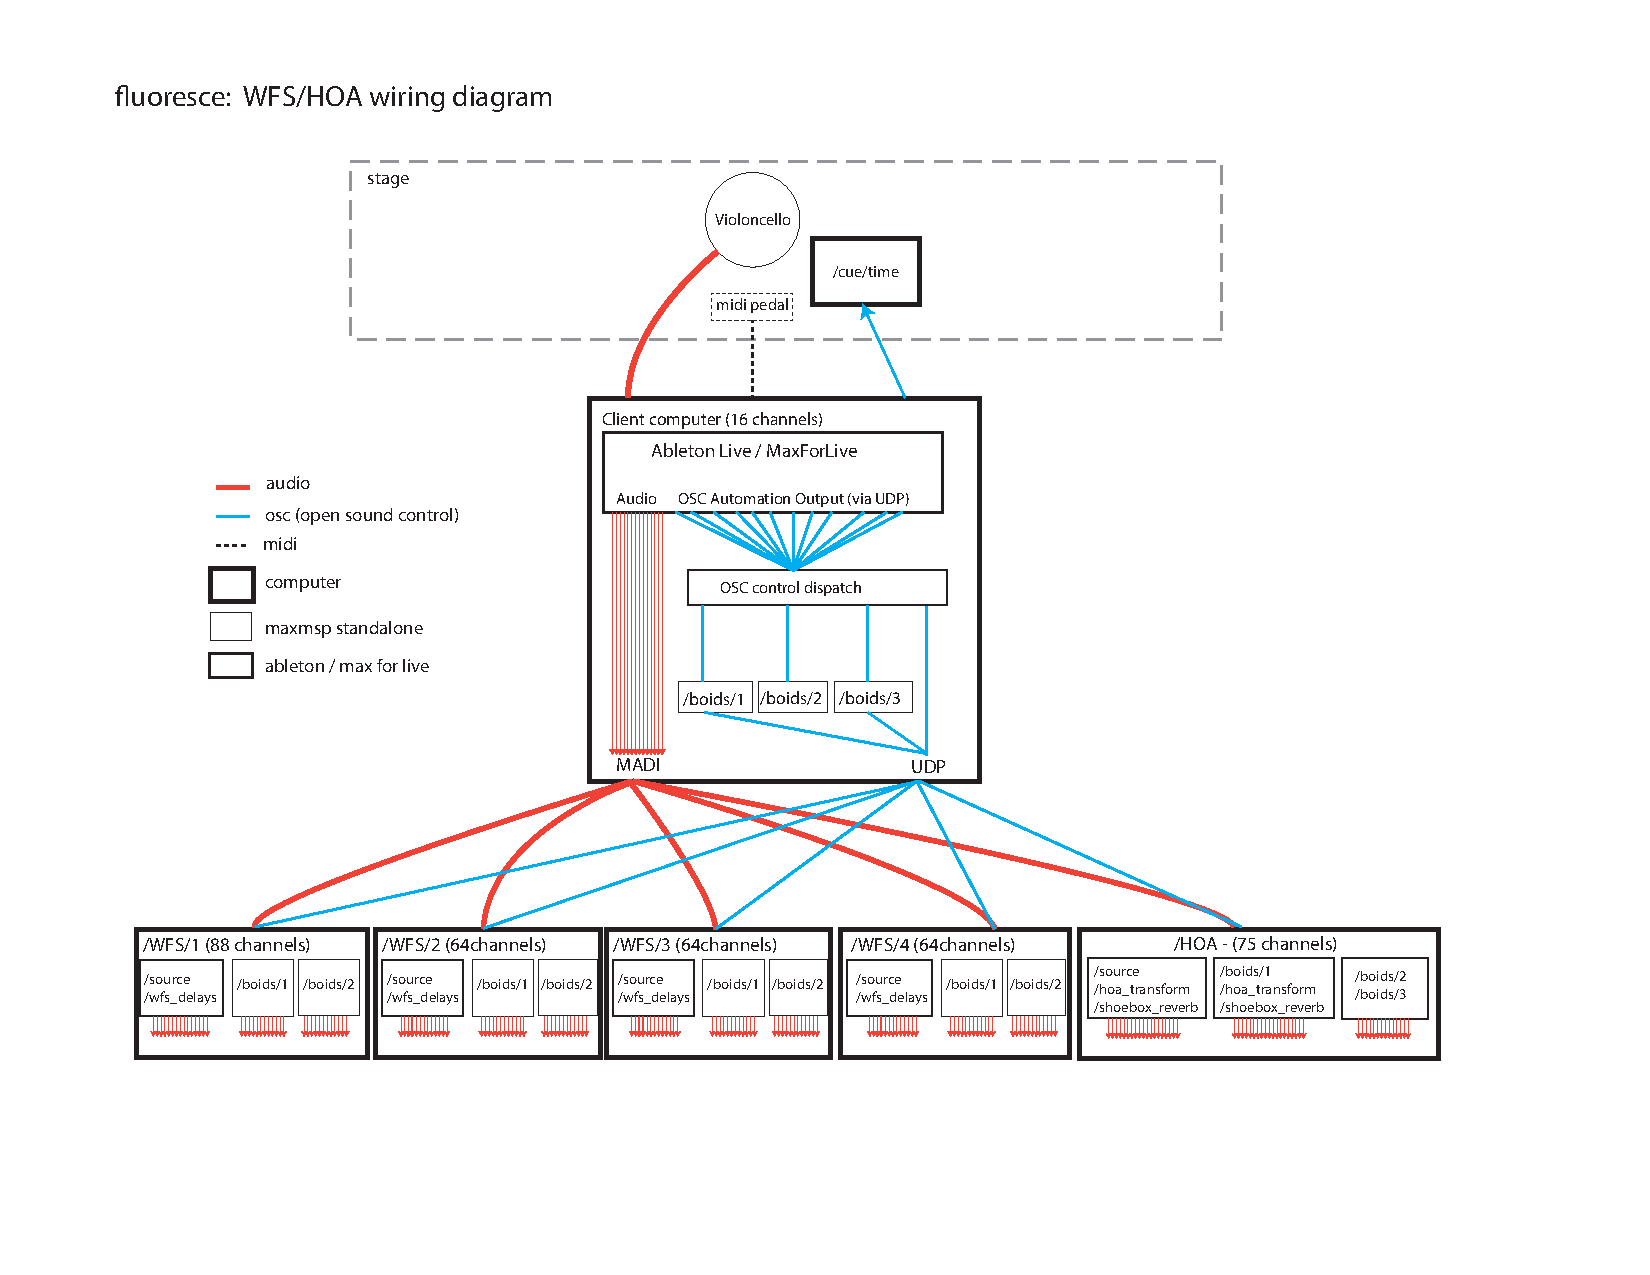
\includepdf[
	angle = 90,
	addtolist={1, figure, {Schéma complet de branchement pour la pièce \textit{Fluoresce}, Rama Gottfried, 2012}, fig:schemaInstallationFluoresceComplet}, 
	pagecommand = {\section{Schéma complet de branchement pour la pièce \textit{Fluoresce}, Rama Gottfried, 2012}\label{sec:schemaInstallationFluoresceComplet}}]{Annexes/schemaInstallationFluoresceComplet.pdf}

\section{Deux transcriptions de la pièce \textit{Reflets de l'ombre}, Carmine E. Cella, 2013}
\label{sec:refletsDeLOmbre}
\begin{figure}[H]
	\centering
	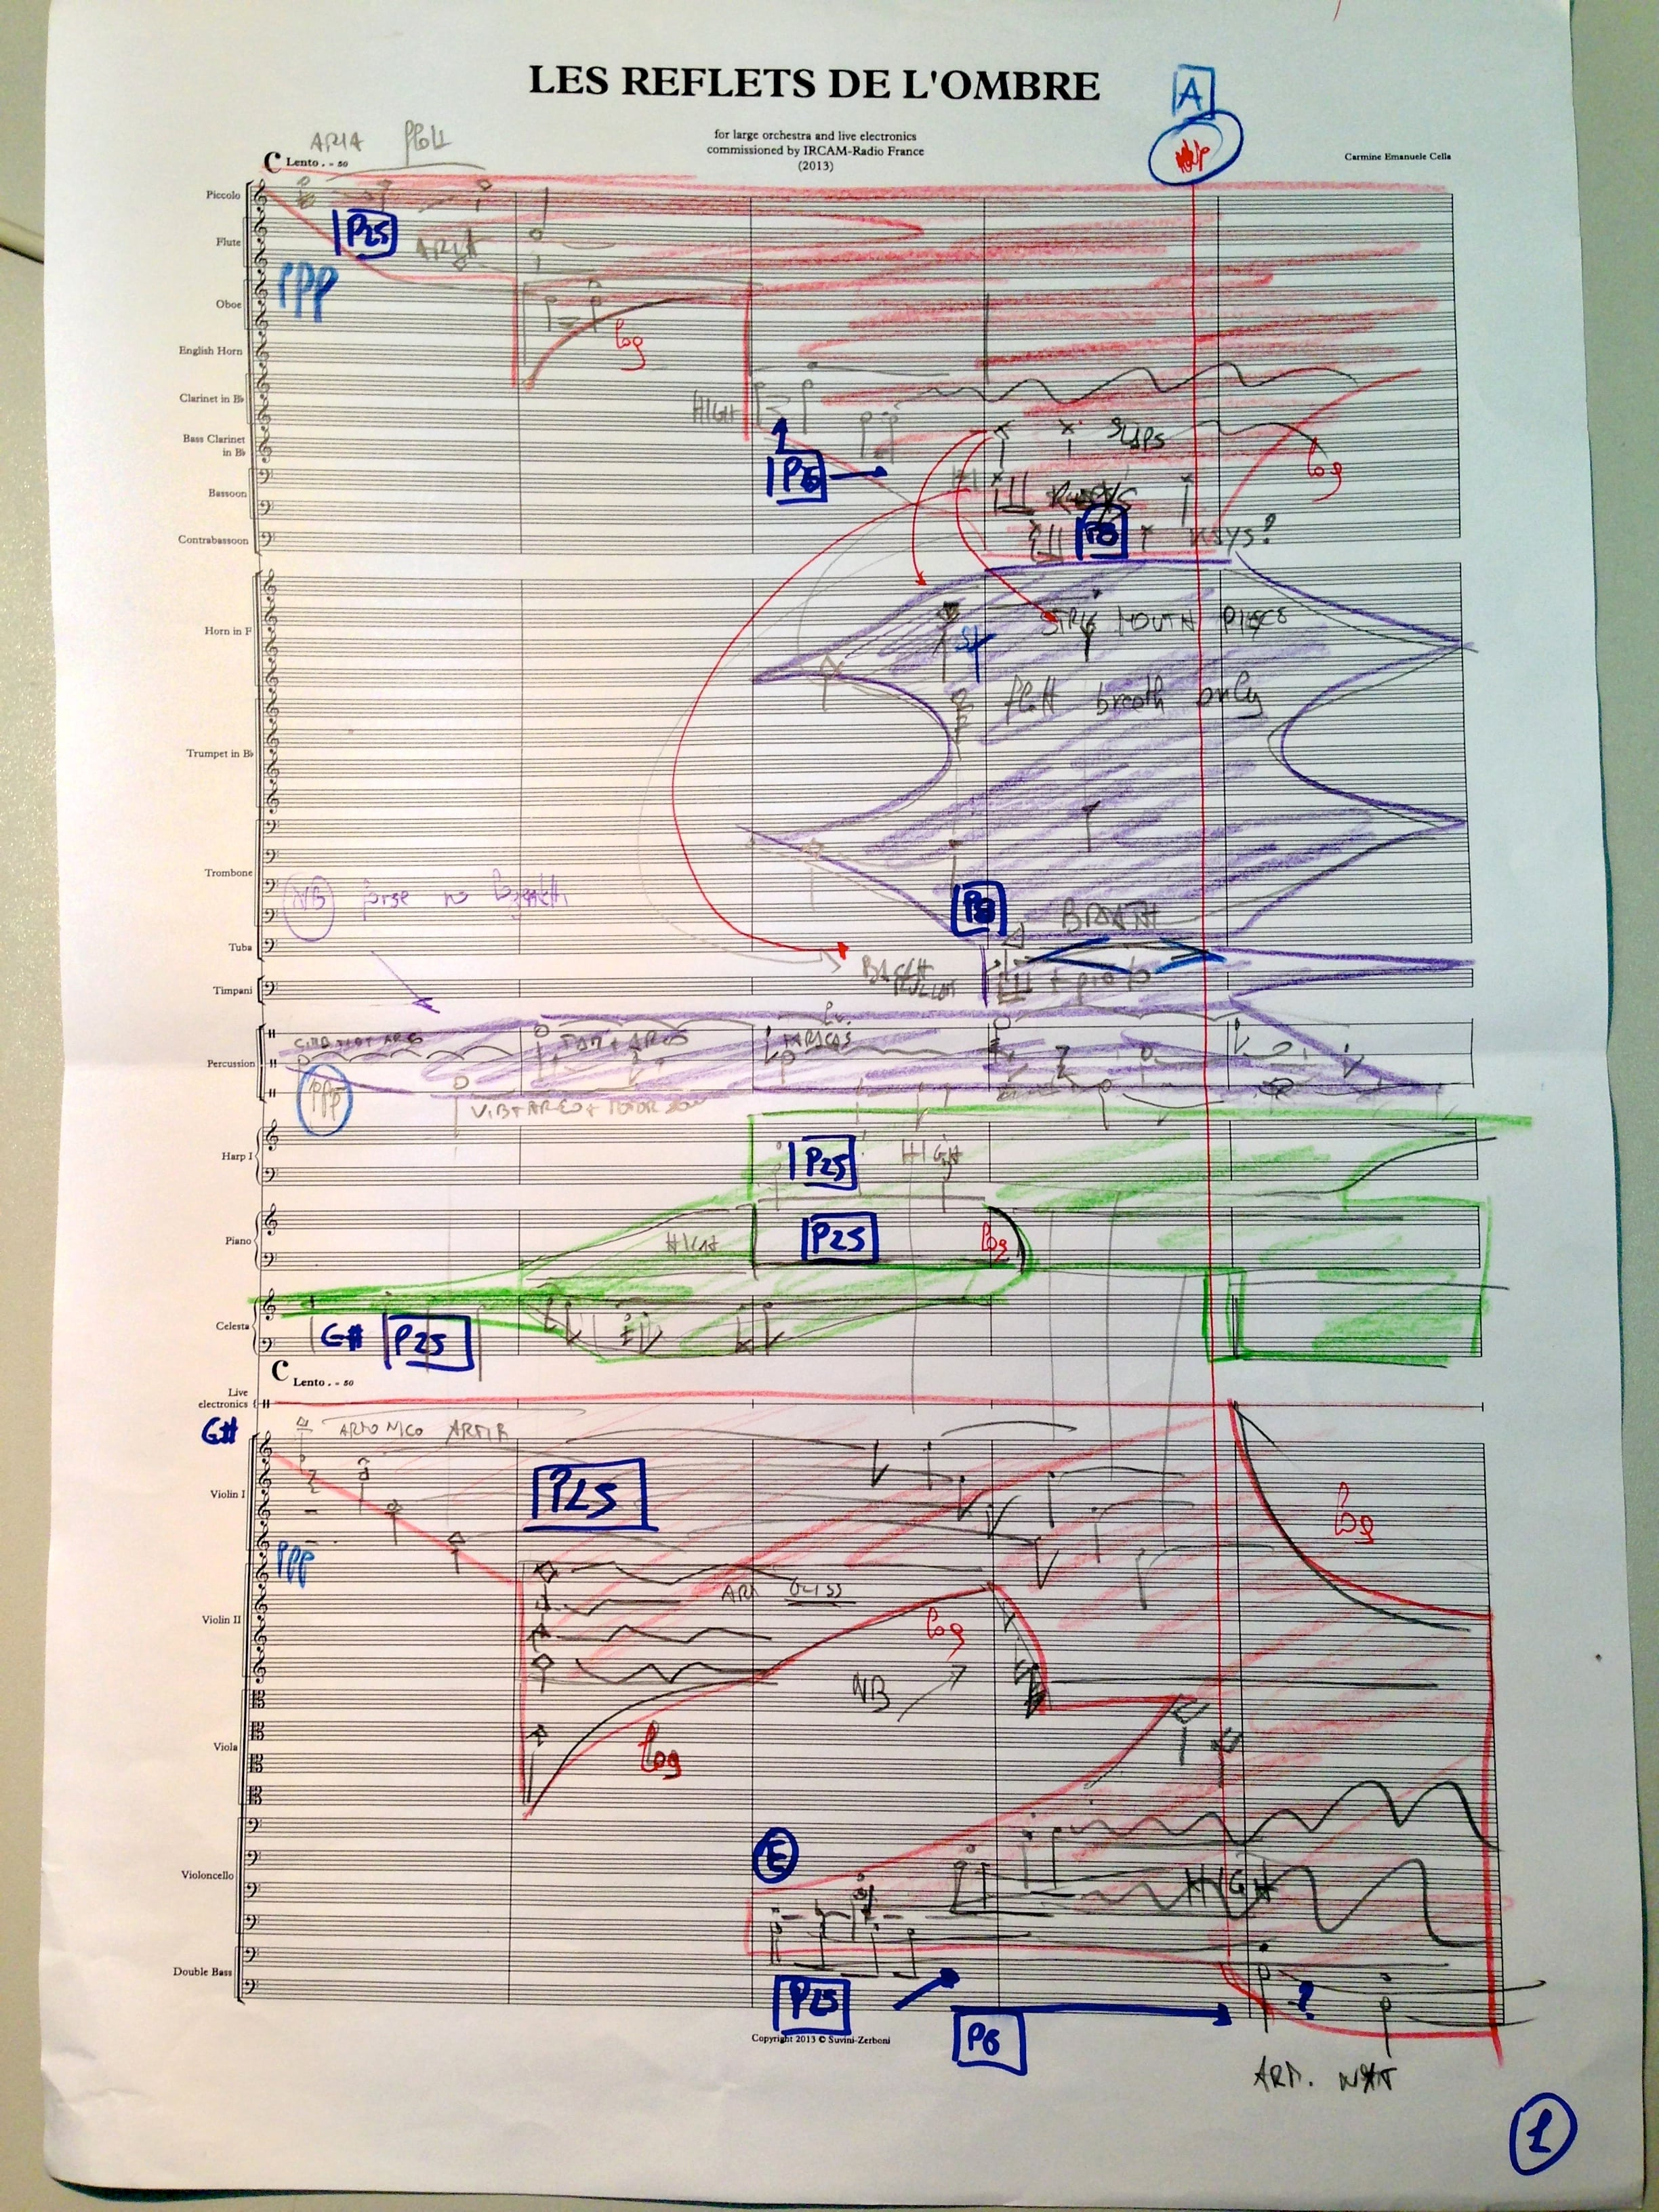
\includegraphics[keepaspectratio=true, width=0.9\textwidth]{Annexes/i/refletsDeLOmbreFantaisie.jpg}
	\caption{Extrait d'une première version de \textit{Reflets de l'ombre} par Carmine E. Cella}
	\medskip
	\small
	\textit{Cette première version représente la pièce en termes de variations du timbre du son.
	La musique y est notée de manière quasi morphologique, avec quelques ajouts de symboles de la gravure standard.}	
	\label{fig:refletsDeLOmbreFantaisie}
\end{figure}

\begin{figure}[H]
	\centering
	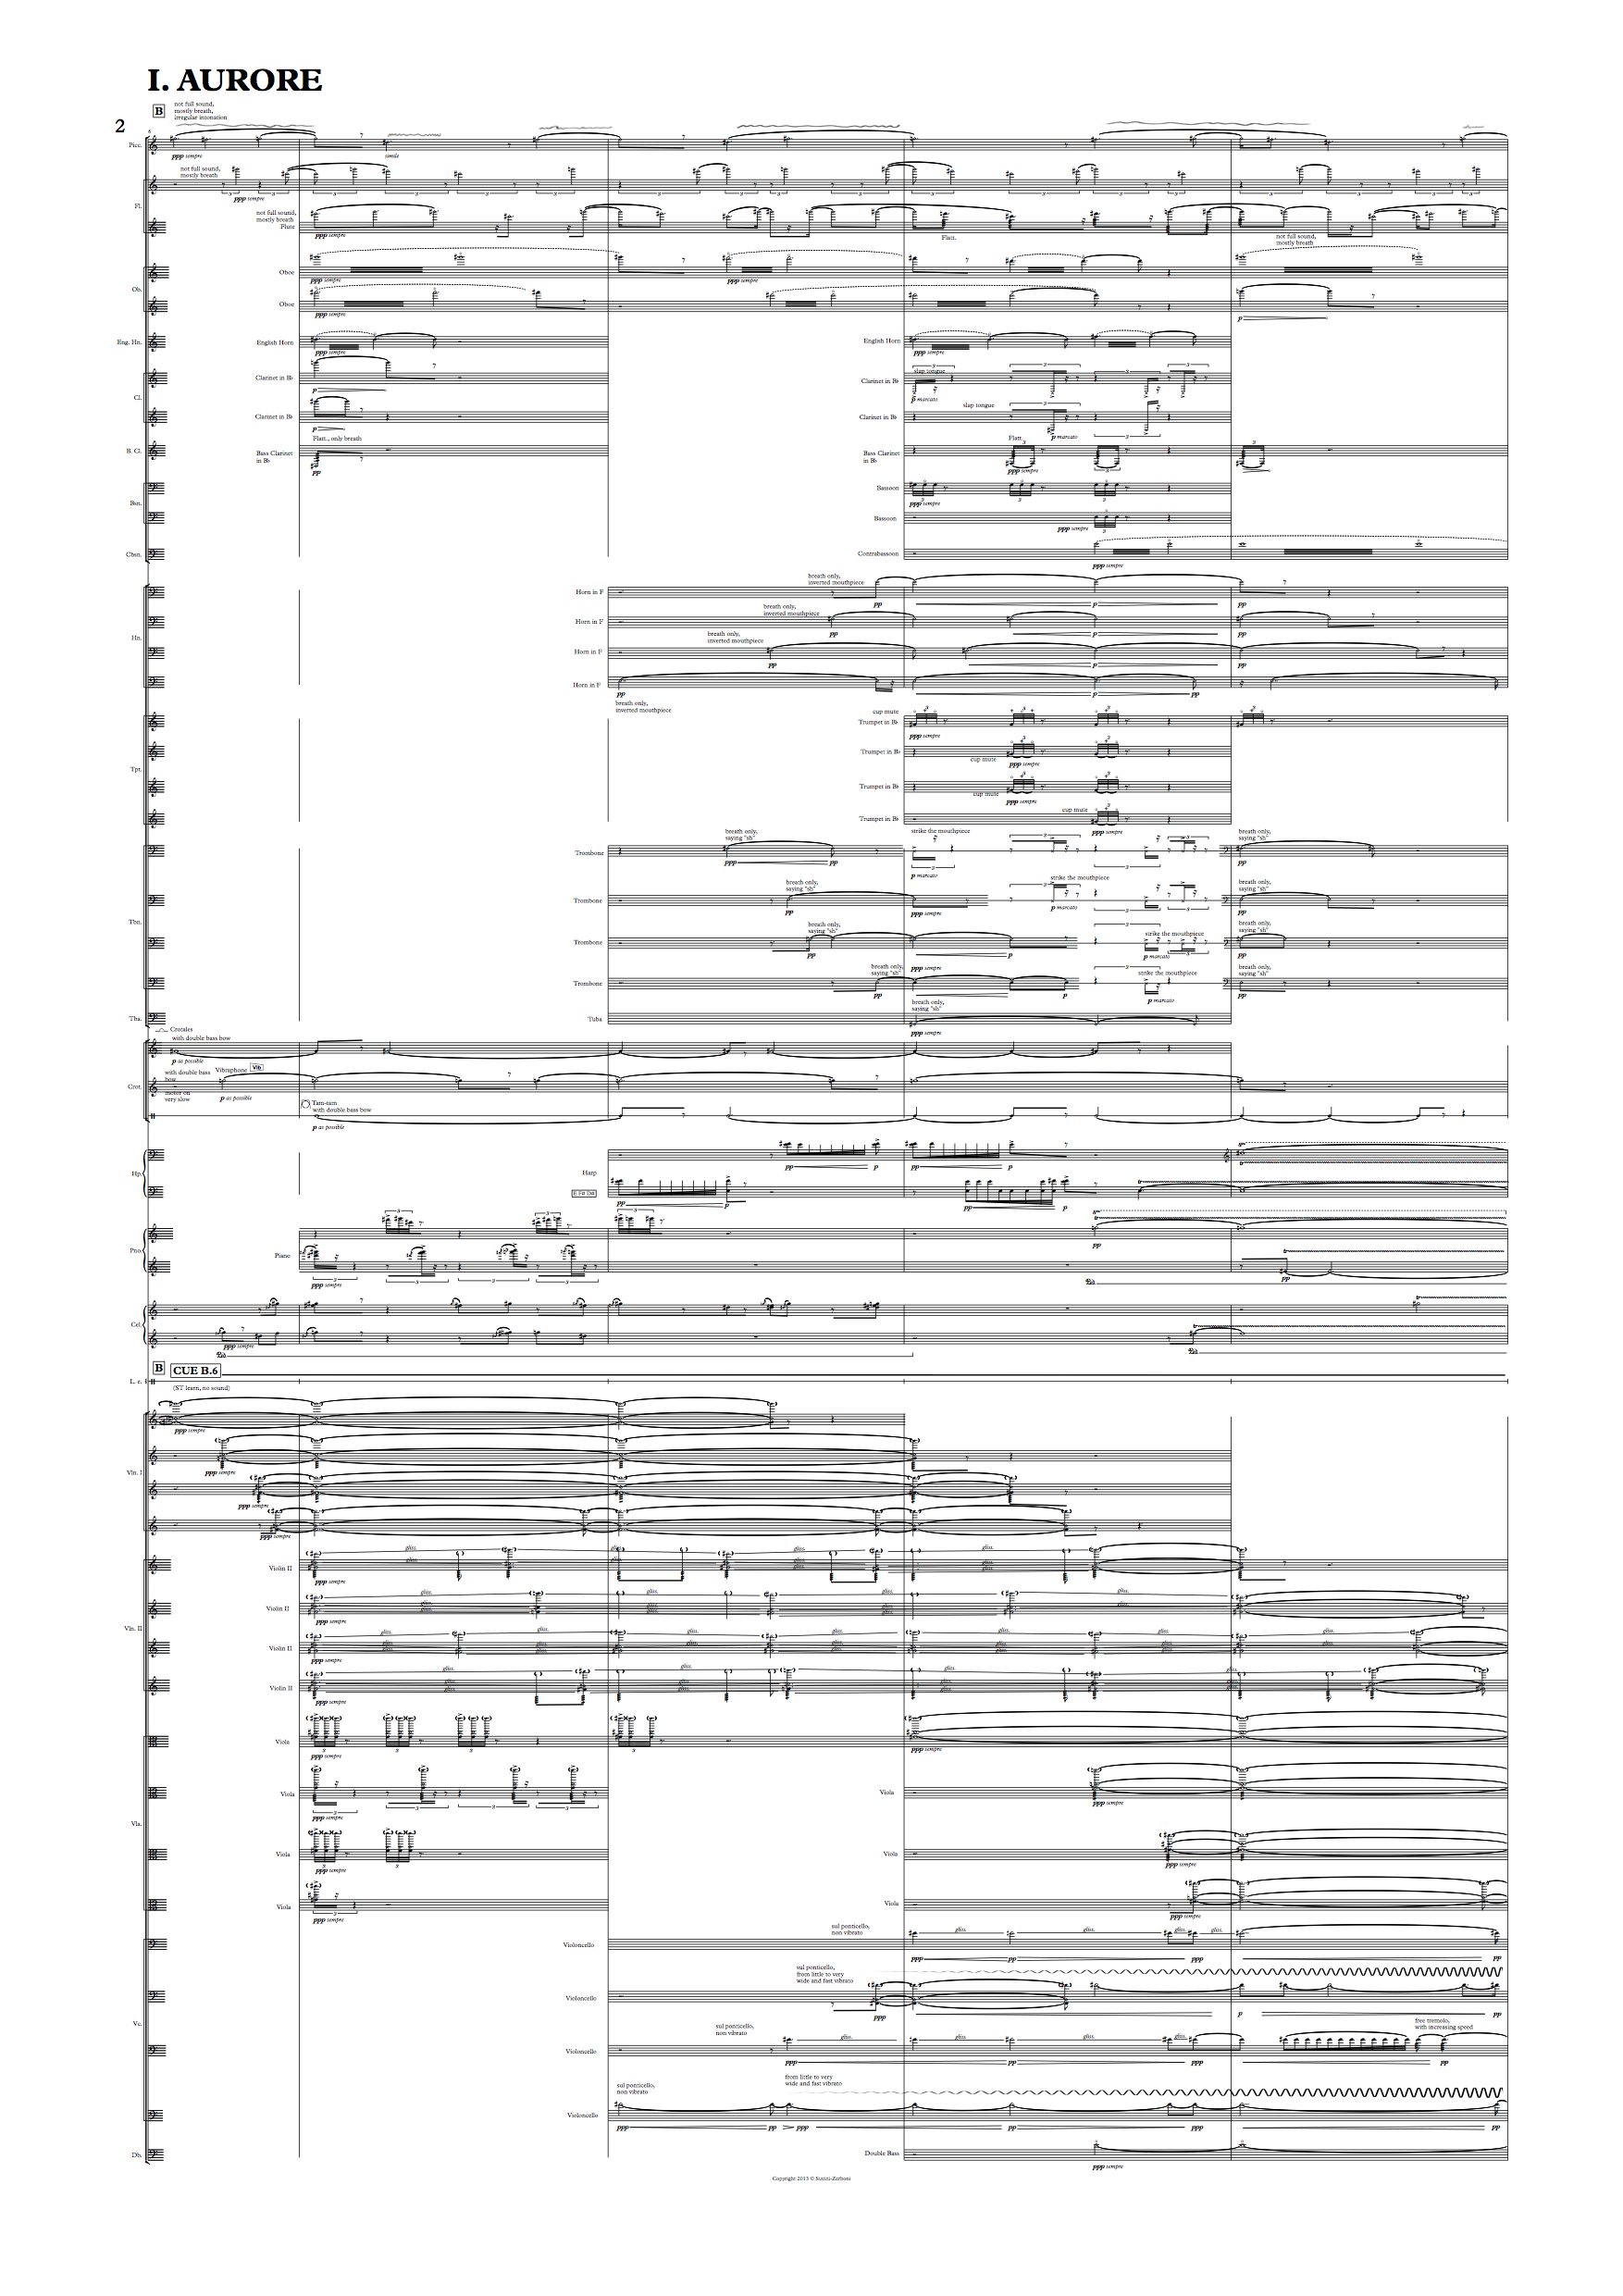
\includegraphics[keepaspectratio=true, width=\textwidth]{Annexes/i/refletsDeLOmbreReel.png}
	\caption{Extrait d'une version éxecutée par un orchestre de \textit{Reflets de l'ombre} par Carmine E. Cella}
	\medskip
	\small
	Cette version de la pièce, qui est destinée à l'orchestre exécutant, a été remaniée vis à vis de la version de la figure \ref{fig:refletsDeLOmbreFantaisie}. Cependant, les formes du son se retrouvent même dans cette transcription plus littérale. 	
	\label{fig:refletsDeLOmbreReel}
\end{figure}
\clearpage

\section{Fragment de la pièce \textit{Lucky Wok}, Mike Solomon}
\label{sec:luckyWokSolomon}
\begin{figure}[H]
	\centering
	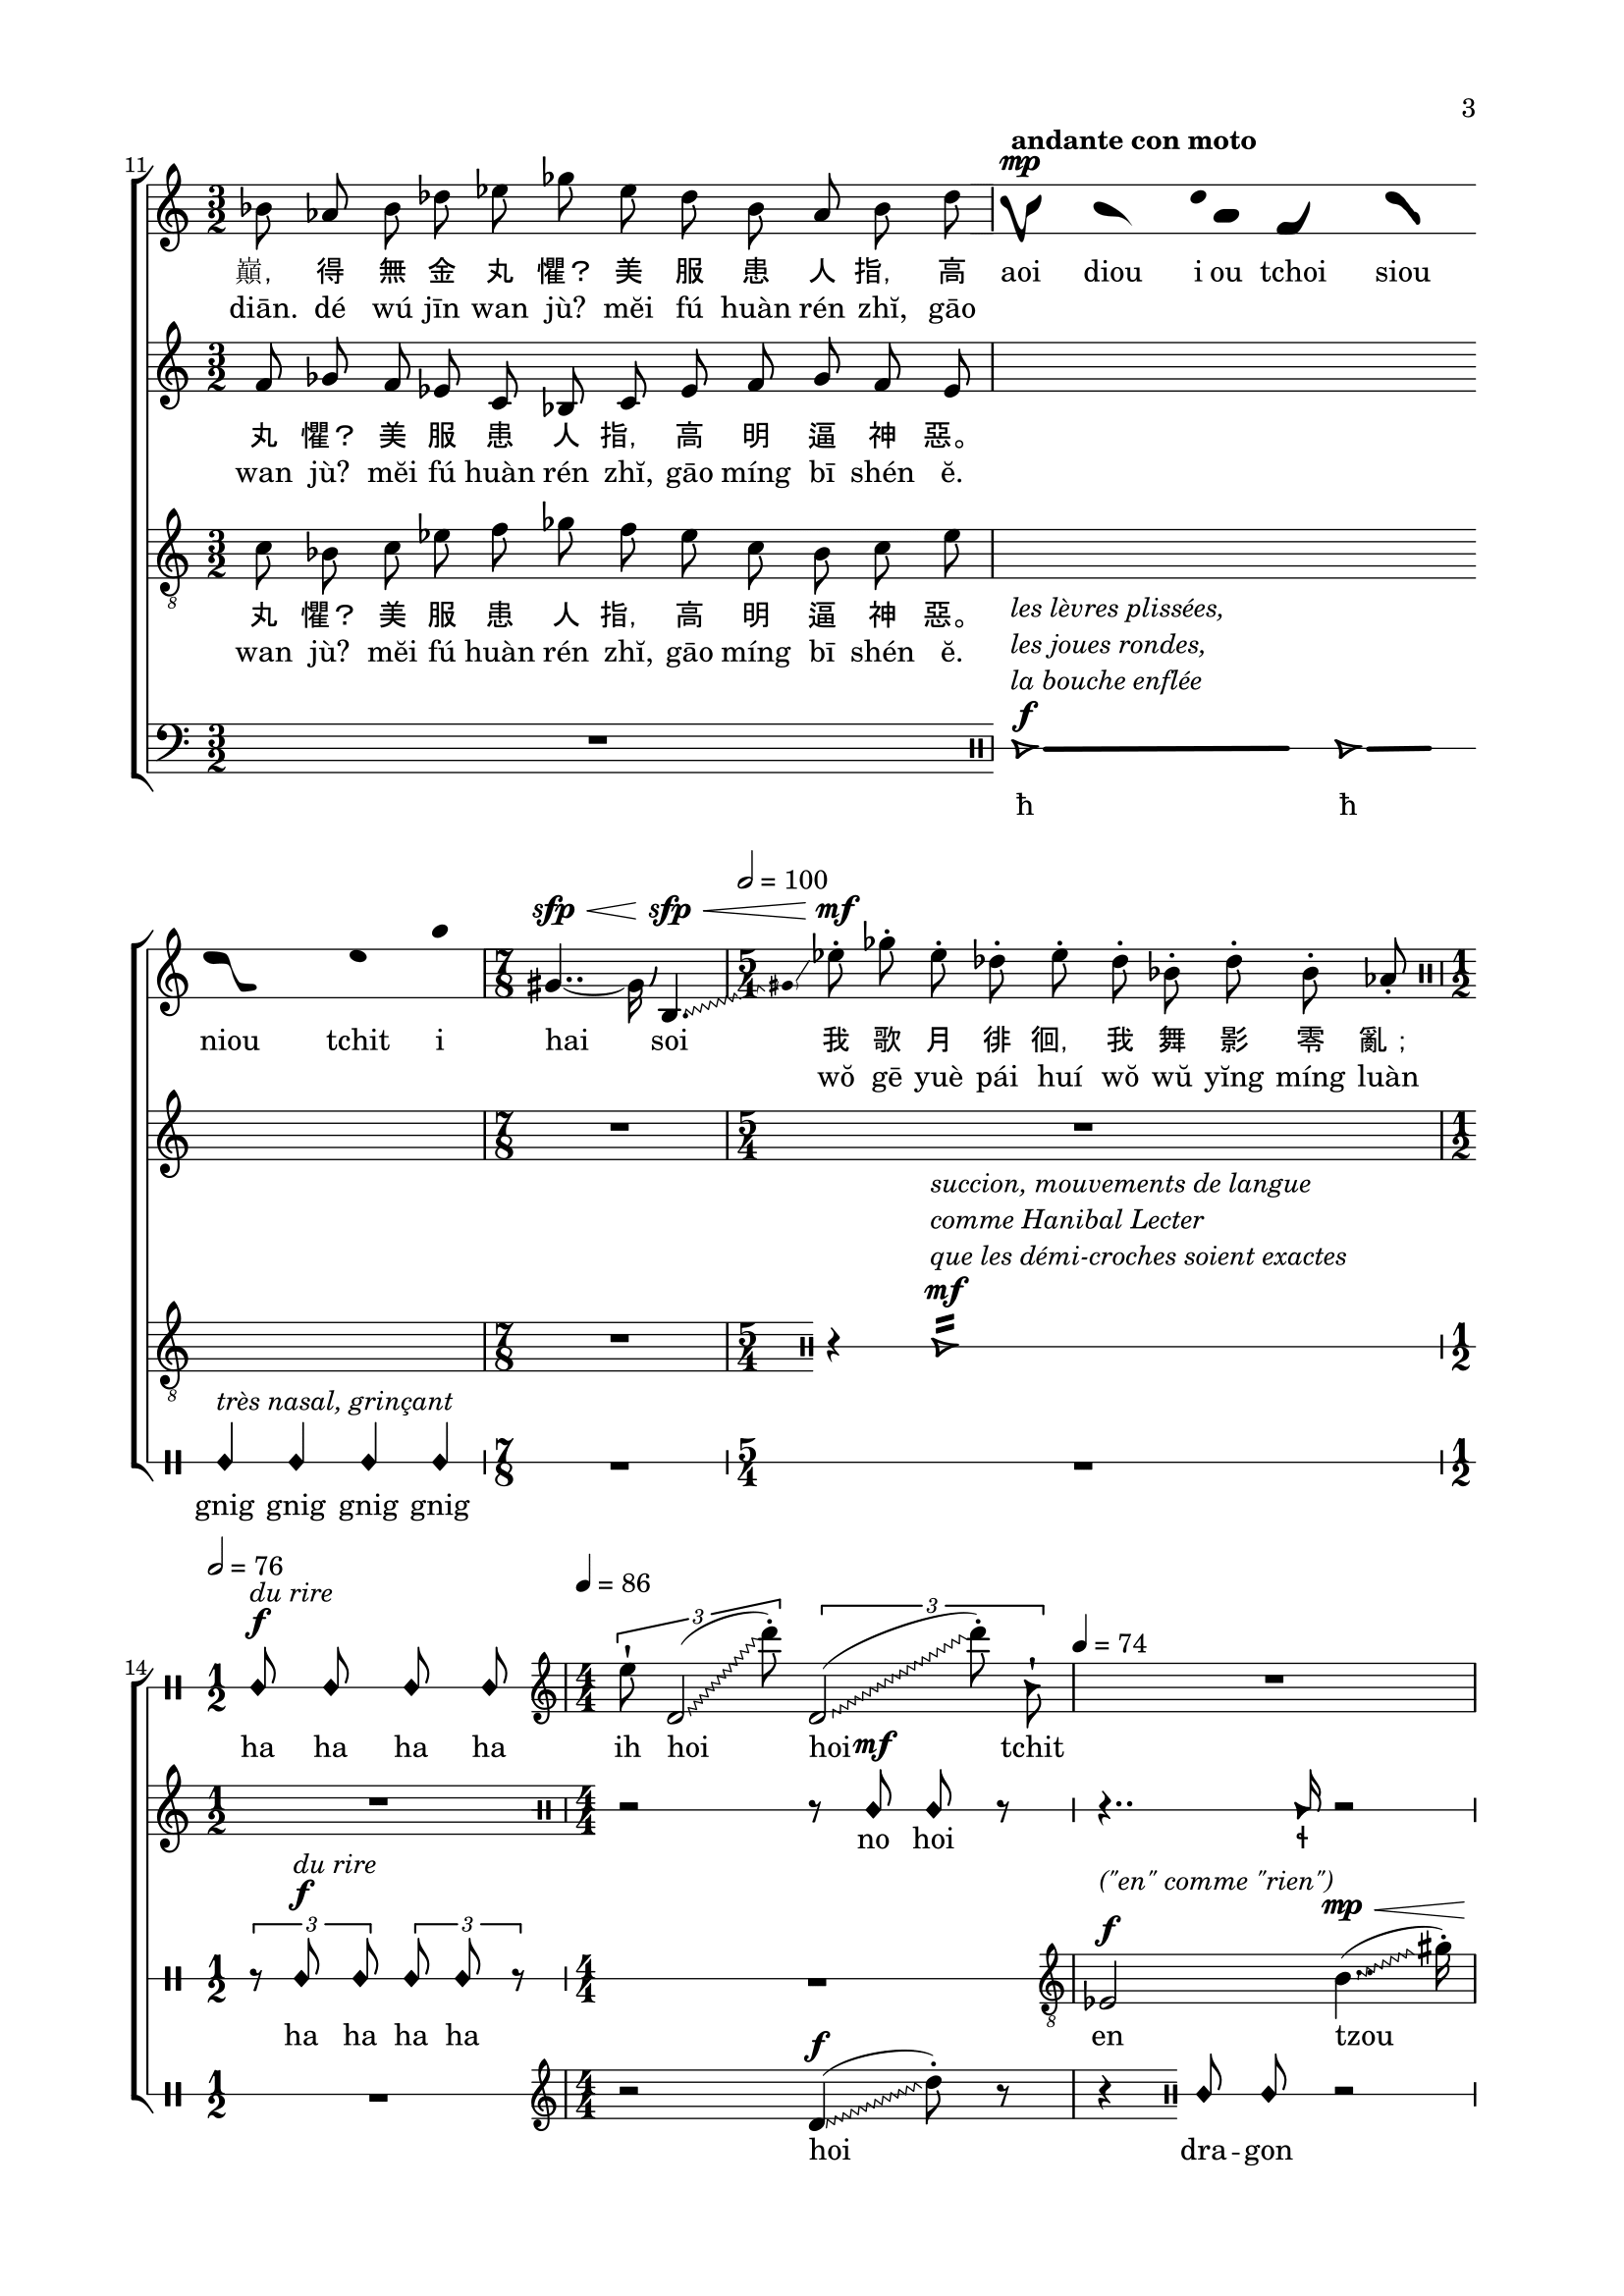
\includegraphics[keepaspectratio=true, width=0.92\textwidth]{Annexes/i/lucky.png}
	\caption{Fragment de la pièce \textit{Lucky Wok}, Mike Solomon}
	\medskip
	\small
	\it
	L'ensemble des symboles et effets de la partition sont produits avec Lilypond. 	
	\label{fig:luckyWokSolomon}
\end{figure}

\section{Exemple de partition créée avec IanniX}
\label{sec:exemplePartitionIannix}
\begin{figure}[H]
	\centering
	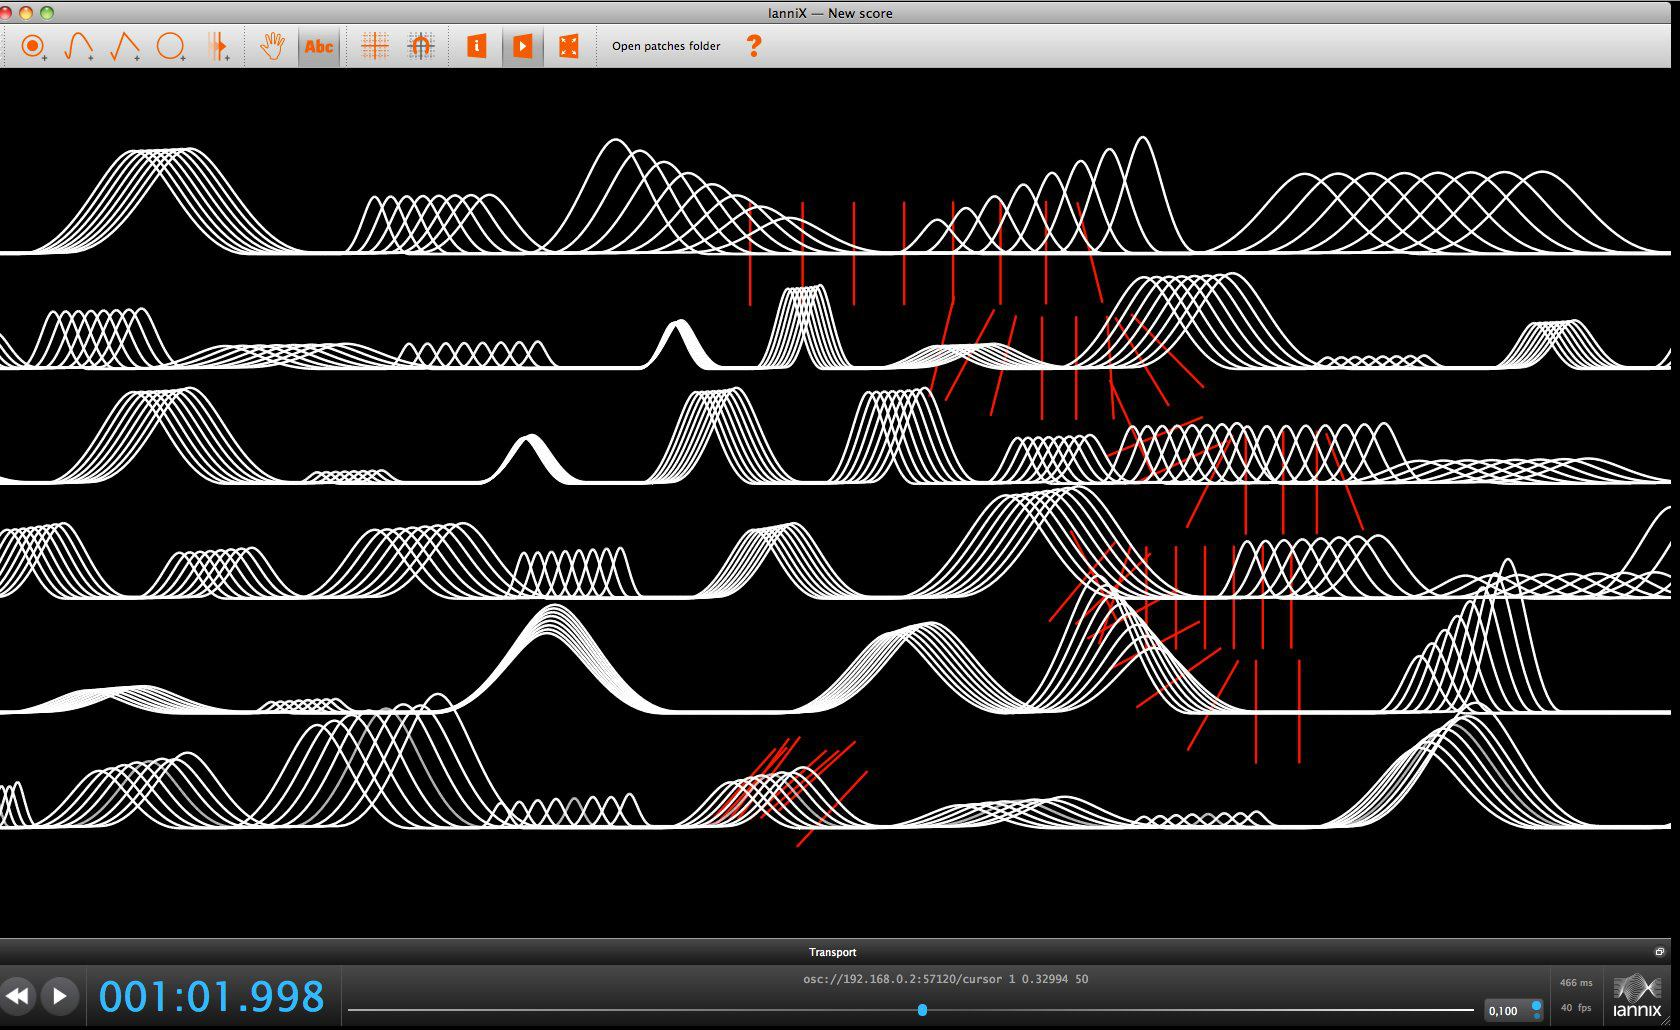
\includegraphics[keepaspectratio=true, width=0.92\textwidth]{Annexes/i/exemplePartitionIannix.jpg}
	\caption{Exemple de partition créée avec IanniX}
	\medskip
	\small
	\it
	Les barres rouges représentent les curseurs avançant le long des courbes blanches.
	Le caractère continue des courbes et leur superposition fait penser à une description morphologique de l'onde sonore. -- Source : Blog de Nicolas Boillot, \url{https://www.fluate.net/code/tools/} 	
	\label{fig:exemplePartitionIannix}
\end{figure}

\section{Exemple de partition interactive avec i-score}
\label{sec:exempleIScore}
\begin{figure}[H]
	\centering
	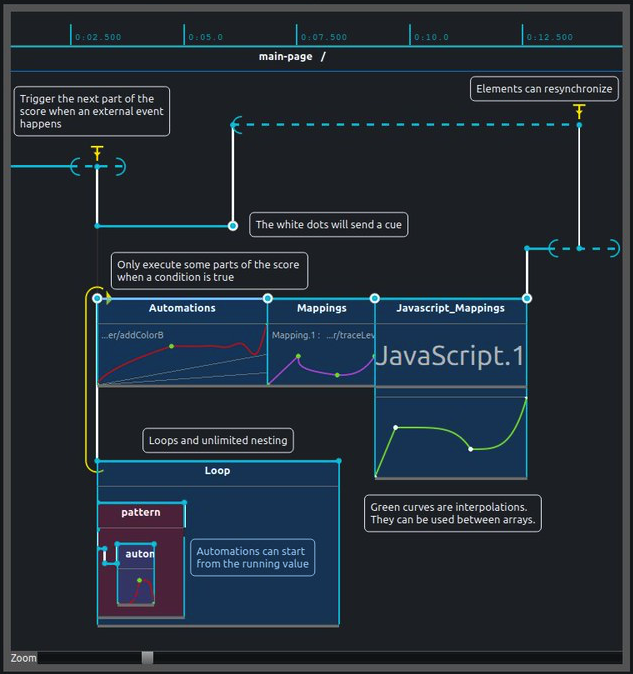
\includegraphics[keepaspectratio=true, width=\textwidth]{Annexes/i/exempleIScore.jpg}
	\caption{Exemple de partition interactive avec i-score}
	\medskip
	\small
	\it  	
	\label{fig:exempleIScore}
\end{figure}

\section{Vue de l'interface graphique de EAnalysis}
\label{sec:exempleVueEAnalysis}
\begin{figure}[H]
	\centering
	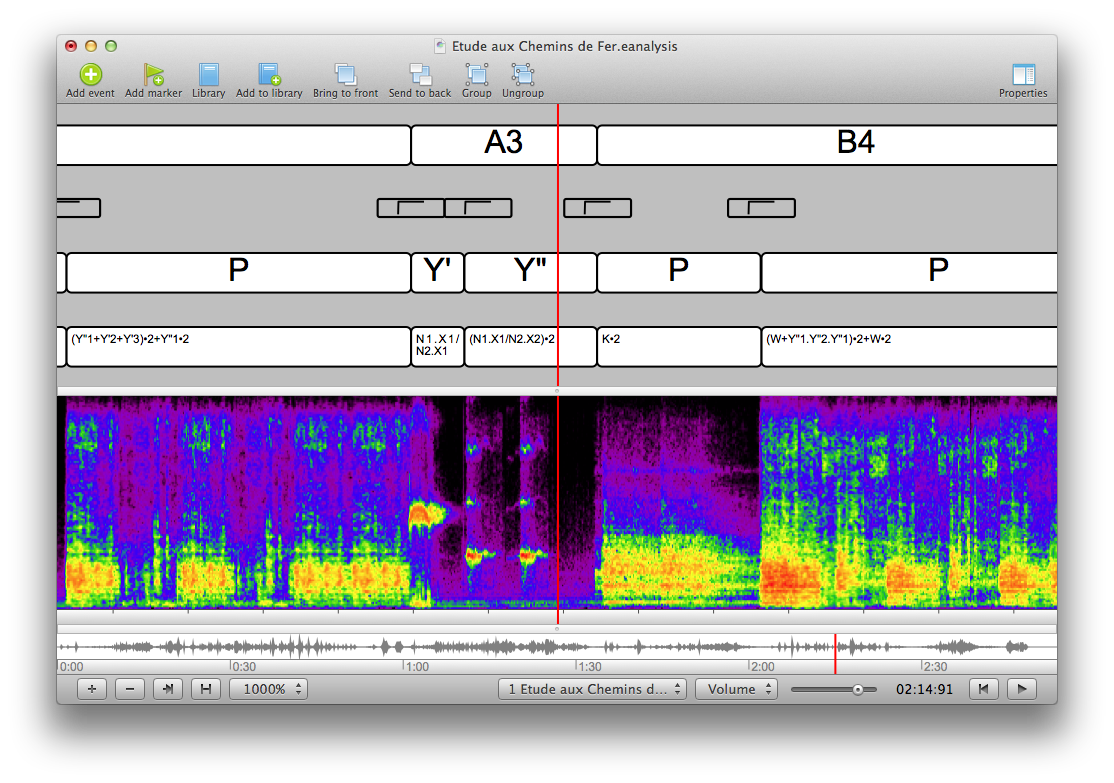
\includegraphics[keepaspectratio=true, width=0.92\textwidth]{Annexes/i/exempleVueEAnalysis.png}
	\caption{Vue de l'interface graphique de EAnalysis}
	\medskip
	\small
	\it
	Plusieurs vues de la pièce \textit{Étude aux Chemins de Fer} dans l'environnement \textit{EAnalysis}.
	De bas en haut : au premier niveau, la vue sous forme d'ondes; au deuxième niveau, le spectrogramme; au troisième niveau, la présentation des graphic et analytic events sur une ligne de temps parallèle.  	
	\label{fig:exempleVueEAnalysis}
\end{figure}